\section{Delay \& Sum Algorithmus}

	Der Delay \& Sum Algorithmus ist eine Möglichkeit, eine akustische Antenne zu implementieren. Der Algorithmus beruht auf der Addition ("Sum") der unterschiedlich verzögerten ("Delay") Eingangssignale einzelner Mikrofone. Dabei müssen ebene Schallwellen und Kugelschallwellen jeweils unterschiedlich behandelt werden. Generell gilt die Annahme, dass sich Antenne und Quelle im Freifeld befinden (also keine Reflexionen vorhanden sind).
	
	In Abbildung \ref{fig:das_basic} ist ein beispielhaftes Mikrofonarray dargestellt, bestehend aus $N$ Mikrofonen $m_1,...,m_N$, die im Abstand von $\Delta x$ in einer Reihe angeordnet sind. Eine Schallquelle $Q$ befindet sich im Winkel $\alpha$ vor dem Array.
	Dieser Winkel führt dazu, dass die Schallwelle jedes Mikrofon mit einer bestimmten Verzögerung $\tau_n$ erreicht.
	Die Summe der Mikrofonsignale $p_n(t)$ ist dann
	\begin{equation}
		s_{sum}(t, \alpha) = \sum_{n=1}^{N} p_n(t - \tau_n(\alpha))
	\end{equation}
	Unter der Annahme, dass der Übertragungsweg von der Quelle zur Summierstelle (Luft, Mikrofon, Kabel) keine Signalveränderungen bewirkt, wird also das selbe Signal mit $N-1$ zeitlich verschobenen Kopien von sich selbst addiert.
	Dadurch kommt es zu Auslöschungen und Abschwächungen, sodass generell $RMS(s_{sum}(t, \alpha=0)) \ge RMS(s_{sum}(t, \alpha \ne 0))$\footnote{$RMS(x(t)) = \sqrt{\frac{1}{T} \cdot \int_{0}^{T} x^2(t) dt }$}.
	
	Die Idee des Delay \& Sum Algorithmus ist nun, die theoretischen Verzögerungszeiten für alle Winkel $\alpha \in [-90^{\circ}, 90^{\circ}]$ zu berechnen und durch nachträgliches "inverses" Verzögern der Mikrofonsignale auszugleichen.
	Anschließend summiert man die diese "invers verzögerten" Signale und sucht den Winkel, unter dem der Effektivwert dieser Summe maximal wird.
	Dieser Winkel wird dann als Schalleinfallsrichtung angenommen.
	
	\begin{figure}[h]
		\begin{center}
		\includegraphics[scale=0.3]{img/DelaySumDiagram}
		\caption{Beispielhaftes Mikrofonarray mit 8 Mikrofonen mit einer Schalquelle, die eine ebene Welle aus Richtung $\alpha$ emittiert.}
		\label{fig:das_basic}
		\end{center}		
	\end{figure}

\subsection{Delay \& Sum für Ebene Wellen}
	
	Eine Ebene Welle zeichnet sich dadurch aus, dass ihre Wellenfront eine Ebene ist. Die Ausbreitungsrichtung ist also überall gleich.
	Grundsätzlich strahlen "kleine" Quellen (wie zum Beispiel ein Mensch oder ein Lautsprecher) Schall kugelförmig ab. Mit zunehmender Entfernung von der Quelle ähnelt die Schallwelle jedoch immer mehr einer ebenen Welle, sodass ab einer gewissen Distanz von der Schallquelle auch die Annahme einer ebenen Wellenausbreitung getroffen werden kann.
	
	%Skzze ebene Wellen
	Für ebene Wellen stellt sich der Delay \& Sum Algorithmus recht einfach dar. Trifft eine ebene Welle unter dem Winkel $\alpha$ auf das Mikrofonarray, so trifft diese zuerst auf das äußerste Mikrofon und erreicht alle anderen Mikrofone erst nach einer gewissen Verzögerungszeit $\tau_n$.
	Dabei ist speziell für die Annahme ebener Wellen $\tau_n = (n - 1) * \Delta t$. Die Verzögerungszeit zwischen zwei Mikrofonsignalen $\Delta t$ kann mit 
	\begin{equation}
		\Delta t = \frac{\Delta x}{c} = \frac{\Delta x \cdot \sin(\alpha)}{c}
	\end{equation}
	berechnet werden, wobei $c = 340 \frac{m}{s}$ für die Schallgeschwindigkeit in Luft angenommen wird.
	Das Ausgangssignal des Arrays für einen Winkel $\alpha$ berechnet sich dann mit
	\begin{equation}
		s = \sum_{n=1}^{N} p_m(t - \tau_n(\alpha))
		\label{eq:das_plane}
	\end{equation}
	
	Trägt man den Effektivwert des Arraysignals über dem Winkel auf, so ergibt sich die Richtungsfunktion des Arrays. In Abbildung \ref{fig:bsp_plot} ist beispielhaft die Richtungsfunktion für eine Quelle bei $\alpha = 15^{\circ}$ dargestellt.
	Das Maximum der Effektivwerte ist deutlich bei 15\textdegree\ erkennbar.
	
	\begin{figure}[h]
		\begin{center}
			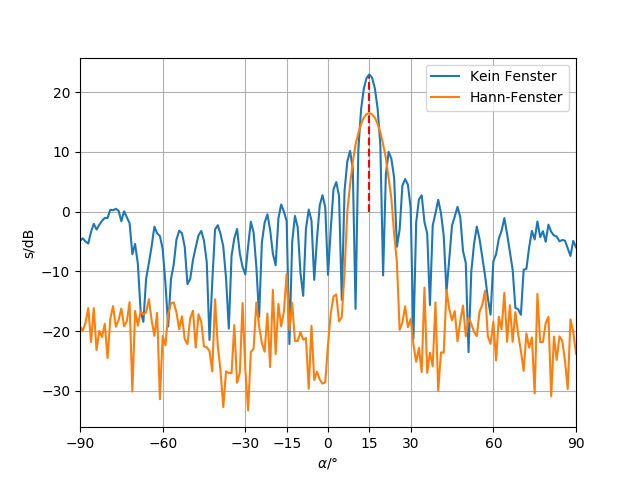
\includegraphics[scale=0.7]{img/bsp_plot_15_beides.png}
			\captionsetup{justification=centering}
			\caption{Richtungsfunktion für eine Quelle bei $\alpha=15^{\circ}$ mit und ohne Gewsichtung. \\
				Das Quellsignal ist ein Sinus mit $f=1000Hz$, das Array hat 20 Mikrofone mit $\Delta x = 0.2m$.\\
				Zum Einsatz kam der Algorithmus für ebene Wellen.}
			\label{fig:bsp_plot}
		\end{center}
	\end{figure}

\subsection{Algorithmus für Kugelwellen}

	\begin{figure}[h]
		\begin{center}
			\includegraphics[scale=0.3]{img/PointSourceDiagram}
			\captionsetup{justification=centering}
			\caption{Situation für Punktschallquellen: Alle möglichen Quellpositionen liegen auf einer Gerade im Abstand $d$ vor dem Mikrofonarray}
		\end{center}
	\end{figure}

	Für Kugelquellen gestalltet sich die Berechnung der inversen Delays etwas komplizierter. Da der Abstand der Quelle zur Arrayachse $d$ für die Berechnung eine Rolle spielt, muss dieser bekannt sein. Der Algorithmus "probiert" dann wieder eine Reihe von Winkeln durch, wobei sich für jeden Winkel ein Punkt $\vec{p}_{\alpha}$ auf einer zur Arrayachse parallelen Geraden im Abstand $d$ mit
	\begin{equation}\vec{p}_{\alpha} = 
		\begin{pmatrix}
			\tan(\alpha) * d \\
			d
		\end{pmatrix}
	\end{equation}
	ergibt. Sollte sich eine Quelle dort befinden, so ist ihre Entfernung zum Mikrofon $m_n$
	\begin{equation}
		r_n = \lvert \vec{p}_{\alpha} - \vec{p}_{n} \rvert
	\end{equation}
	mit
	\begin{equation}
		\vec{p}_n =
		\begin{pmatrix}
			\frac{L}{2} - \Delta x \cdot (n - 1) \\
			0
		\end{pmatrix}
	\end{equation}
	wobei $L$ die Länge des Arrays ist. Die Zeit $\tau_{\alpha, n}$, die eine Schallwelle braucht, um diesen Abstand zurückzulegen kann mit $\tau_{\alpha, n} = \frac{r_n}{c}$ berechnet werden. Werden alle $\tau_{\alpha, n}$ entsprechend ausgeglichen, so ergibt sich für die tatsächliche Quellenposition (beziehungswese für den Winkel, der dieser entspricht) wieder ein Maximum im Effektivwert des Summensignals aller Mikrofone. Es kann so wie für die Annahme ebener Wellen eine Richtungsfunktion bestimmt werden.
	
	Ein wichtiger Unterschied zum Algorithmus für ebene Wellen besteht darin, dass nicht mehr alle Werte in $[-90^{\circ}, 90^{\circ}]$ für $\alpha$ erlaubt sind, da für betraglich große Winkel das betrachtete Stück der Quellengerade unendlich lang wird. In der vorliegenden Implementierung wird deshalb ein maximaler Betrag für $\alpha$ eingeführt, der einer Quellenposition von 
	\begin{equation}
		\vec{p}_q = 
	\begin{pmatrix}
		\pm L \\
		d
	\end{pmatrix}
	\end{equation}
	entspricht. Damit geht einher, dass der erlaubte Wertebereich von $\alpha$ bei größeren Entfernung zur Quelle kleiner wird.
	

\subsection{Gewichtung der Mikrofone}

	Die Richtungsfunktion lässt sich durch eine Gewichtung der einzelnen Mikrofonsignale verschieden formen. In Abbildung \ref{fig:bsp_plot} ist eine Richtungsfunktion mit und ohne Gewichtung zu sehen.
	Zur Gewichtung der Mikrofone wurde hier die Hann-Fensterfunktion verwendet.
	Man erkennt, dass das Hauptmaximum deutlich verbreitert wurde, während die Nebenmaxima abgesenkt wurden.
	Je nach Anwendungsfall empfehlen sich verschiedene Fensterfunktionen. Sollen zum Beispiel mehrere Quellen, die eng beieinander liegen, erkannt werden, so wird ein schmaleres Hauptmaximum benötigt\footnote{Möser (Hrsg.), Messtechnik der Akustik, Springer 2010, S. 374ff}.